\chapter{Protocollo Diffie-Hellman}
\section{Spiegazione}
\[\boxed{\text{Non è un cifrario, è solo un protocollo per lo scambio della chiave}}\]
Questo protocollo permette la creazione di una chiave di sessione nella quale entrambi i lati partecipano in egual misura. Non è un protocollo di scambio di chiavi, la chiave non viaggia mai: si scambiano informazioni che permettono la costruzione della chiave (ogni volta si mettono insieme informazioni private di un interlocutore). Il protocollo ricorre all'algebra modulare e basa la sua sicurezza sul problema del logaritmo discreto.
\paragraph{Passi} 
\begin{itemize}
	\item \textbf{Primo step}. Alice e Bob si accordano pubblicamente su un numero $p$ primo molto grande ($\approx 1000$ bit) ed un generatore $g$ di $Z_p^*$. Ricordiamo che
	$$Z_p^*=\{1,2, \dots, p-1\}$$
	che posso esprimere nel seguente modo, grazie al generatore $g$
	$$Z_p^*=\{g^k \text{ mod }p, 1 \leq k \leq p-1\}$$
	Ricordarsi che lavorare con un numero primo garantisce l'esistenza di \textbf{\underline{ALMENO}} un generatore di $Z_p^*$
	\item \textbf{Individuazione del generatore}. Non esistono algoritmi deterministici per individuare generatori (si usano algoritmi randomizzati). Nel caso in cui Alice e Bob non abbiano la potenza computazionale per ottenere $<g,p>$ allora utilizzeranno coppie note, per esempio quelle raccomandate dalle linee guida del NIST: vedremo che ciò non è un problema, nella dimostrazione della correttezza supporremo che la coppia sia nota al crittoanalista.
	\item \textbf{Step successivi}. L'algoritmo prosegue un questo modo:
	\begin{itemize}
		\item Alice sceglie $x$ tale che $1 < x < p-1$ e calcola
		$$ A = g^x \text{ mod } p $$
		ed invia $A$ a Bob
		\item Bob sceglie $y$ tale che $1 < y < p-1$ e calcola
		$$ B = g^y \text{ mod } p $$
		ed invia $B$ ad Alice
		\item Alice calcola la chiave di sessione:
		$$ K = B^x \text{ mod } p = \boxed{g^{x \cdot y} \text{ mod } p} $$
		\item Bob calcola la chiave di sessione:
		$$ K = A^y \text{ mod } p = \boxed{g^{x \cdot y} \text{ mod } p} $$
	\end{itemize}
	Entrambi hanno ottenuto lo stesso numero $K$.
	
\end{itemize}
\section{Sicurezza del problema del logaritmo discreto}
\subsection{Attacchi passivi}
Il crittoanalista conosce il numero primo $p$, il generatore $g$, i valori $A$ e $B$.
Per calcolare la chiave di sessione $k[\text{session}]$ bisogna trovare $x$ ed $y$:
\[
    \begin{cases}
    A = g^x \text{ mod } p \\
    B = g^y \text{ mod } p
    \end{cases}
\]
siamo di fronte al problema del \textbf{logaritmo discreto}! Possiamo solo eseguire un forza bruta ma se $p$ è molto grande {\underline{allora c'è poco da fare}}.

\subsection{Attacchi attivi}
\begin{center}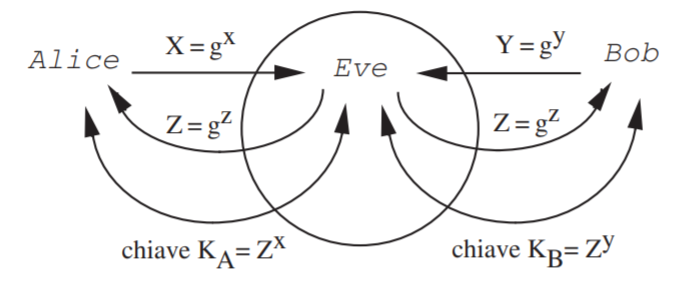
\includegraphics[scale=.6]{images/27.PNG}\end{center}
Diffie-Hellman è vulnerabile agli attacchi di tipo \emph{man-in-the-middle}. Abbiamo Eve che si finge Alice agli occhi di Bob e Bob agli occhi di Alice:
\begin{itemize}
    \item Alice invia $ A = g^x \text{ mod } p$. Eve intercetta $A$ e lo sostituisce con $$E = g^z \text{ mod } p$$
    Bob riceve $E$.
    \item Bob invia $ B = g^y \text{ mod } p $. Eve intercetta $B$ e lo sostituisce con $$E = g^z \text{ mod } p$$
    Alice riceve $E$.
    \item Eve calcola:
    \begin{itemize}
        \item $K_A = A^z \text{ mod } p = g^{x \cdot z} \text{ mod } p$ per parlare con Alice
        \item $K_B = B^z \text{ mod } p = g^{y \cdot z} \text{ mod } p$ per parlare con Bob
    \end{itemize}
    \item Alice calcola $K_A = E^x \mod p$ per parlare con Bob, ma in realtà parlerà con Eve
    \item Bob calcola $K_B = E^y \mod p$ per parlare con Alice, ma in realtà parlerà con Eve
\end{itemize}
Qualsiasi cosa che Alice mandi a Bob, Eve può decifrarlo, criptare con la chiave di Bob e re-inviarlo.
Viceversa per i messaggi di Bob verso Alice.
Eve può quindi leggere tutti i messaggi da ambo le parti. 
\paragraph{Soluzione} Per risolvere questo problema si possono usare le \emph{Certification of Authority}, cioè dei certificati digitali con il quale si firmano i valori $A$ e/o $B$.

